\chapter{User Experience}
\label{chap:UX}
The user experience collection was performed after introducing the final version of the system. First was given a a workshop regarding the system use. This decision was taken due to the fact that not all volunteered employees were the target users. Total number of respondents was seven. All of them were from different divisions of the company and had a different background. Three of respondents were from customer support and project management and four from the development team. 

The task for respondents during collection of user experience was to recreate test coverage introduced in the chapter \ref{chap:implementation} for the module \textit{stack} from the same chapter. They were allowed to use their favorite spreadsheet editor.

The scenario was defined in a following way:
\begin{itemize}
	\item Open spreadsheet editor;
	\item Create new spreadsheet;
	\item In the cell \textbf{A1} add the \textit{description} text\textit{ \textbf{User experience}};
	\item In the cell \textbf{A2} add the \textit{file under test} name \textit{\textbf{stack}};
	\item In the cell \textbf{A3} add  \textit{module under test} name \textit{\textbf{stack}};
	\begin{itemize}
		\item In the cell \textbf{B3} add the \textit{method under test} name \textit{\textbf{size}};
		\item In the cell \textbf{D3} add the indicator of \textit{deep comparison}\textit{ \textbf{$||$}};
		\item In the cell \textbf{E3} add the \textit{expected return} value \textit{\textbf{ \{ "size": 0 \} }};
	\end{itemize}
	\item In the cell \textbf{A4} add the \textit{module under test} name\textit{ \textbf{stack}};
	\begin{itemize}
		\item In the cell \textbf{B4} add the \textit{method under test} name  \textit{\textbf{push}};
		\item In the cell \textbf{C4} add the \textit{input parameter} value \textit{\textbf{ \{ "el": 1 \}}};
		\item In the cell \textbf{D4} add the indicator of \textit{deep comparison}\textit{ \textbf{$||$}};
		\item In the cell \textbf{E4} add the \textit{expected return} value\textit{ \textbf{ \{ \} }};
	\end{itemize}
	\item In the cell \textbf{A5} add the  \textit{module under test} name \textit{ \textbf{stack}};
	\begin{itemize}
		\item In the cell \textbf{B5} add the \textit{method under test} name \textit{\textbf{top}};
		\item In the cell \textbf{D5} add the indicator of \textit{deep comparison}\textit{ \textbf{$||$}};
		\item In the cell \textbf{E5} add the \underline{reference} to the cell \textbf{C4} as an \textit{expected return value};
	\end{itemize}
%	
	\item In the cell \textbf{A6} add the \textit{module under test} name\textit{ \textbf{stack}};
	\begin{itemize}
		\item In the cell \textbf{B6} add the \textit{method under test} name\textit{ \textbf{push}};
		\item In the cell \textbf{C6} add the reference to th cell \textbf{E5} as an \textit{ input parameter};
		\item In the cell \textbf{D6} add the indicator of \textit{schema comparison}\textit{\textbf{ $|$}};
		\item In the cell \textbf{E6} add the \textit{expected return} value\textit{ \textbf{ \{ \} }};
	\end{itemize}
%	
	\item In the cell \textbf{A7} add the \textit{module under test} name\textit{\textbf{ stack}};
	\begin{itemize}
		\item In the cell \textbf{B7} add the \textit{method under test} \textit{\textbf{push}};
		\item In the cell \textbf{C7} add the \underline{reference} to th cell \textbf{E5} as an\textit{ input parameter};
		\item In the cell \textbf{D7} add the indicator of \textit{schema comparison} \textit{\textbf{$|$}};
		\item In the cell \textbf{E7} add the \textit{expected return} value\textit{ \textbf{ \{ \} }};
	\end{itemize}
%	
	\item In the cell \textbf{A8} add the \textit{module under test} name\textit{ \textbf{stack}};
	\begin{itemize}
		\item In the cell \textbf{B8} add the \textit{method under test} name \textit{\textbf{pop}};
		%		\item In the cell \textbf{C6} add the reference to th cell \textbf{E5} as an input parameter
		\item In the cell \textbf{D8} add the indicator of \textit{deep comparison} \textit{\textbf{$||$}};
		\item In the cell \textbf{E8} add the \textit{expected return} value\textit{ \textbf{ \{ "el": 5 \} }};
	\end{itemize}
%	
	\item In the cell \textbf{A9} add the \textit{module under test} name\textit{ \textbf{stack}};
	\begin{itemize}
		\item In the cell \textbf{B9} add the \textit{method under test} name \textit{\textbf{push}};
		\item In the cell \textbf{C9} add the \underline{reference} to th cell \textbf{E8} as an \textit{input parameter};
		\item In the cell \textbf{D9} add the indicator of\textit{ deep comparison}\textit{ \textbf{$||$}};
		\item In the cell \textbf{E9} add the \textit{expected return} value\textit{ \textbf{ \{ \} }};
	\end{itemize}
%	
	\item In the cell \textbf{A10} add the \textit{module under test} name\textit{\textbf{ stack};}
	\begin{itemize}
		\item In the cell \textbf{B10} add the \textit{method under test} name\textit{ \textbf{ pop}};
		%		\item In the cell \textbf{C6} add the reference to th cell \textbf{E5} as an input parameter
		\item In the cell \textbf{D10} add the indicator of \textit{ deep comparison}\textit{ \textbf{$||$}};
		\item In the cell \textbf{E10} add the \underline{reference} to the cell \textbf{E5} as an \textit{expected return value};
	\end{itemize}
%	
	\item In the cell \textbf{A11} add the \textit{module under test} name \textit{\textbf{stack}};
	\begin{itemize}
		\item In the cell \textbf{B11} add the \textit{method under test} name \textit{\textbf{push}};
		\item In the cell \textbf{C11} add the \underline{reference} to th cell \textbf{E10} as an\textit{ input parameter};
		\item In the cell \textbf{D11} add the indicator of \textit{deep comparison}\textit{ \textbf{$||$}};
		\item In the cell \textbf{E11} add the \textit{expected return} value \textit{\textbf{ \{ \} }};
	\end{itemize}
%	
	\item Save the file in to the folder \textit{stack} with name \textit{ux.xlsx};
%	
	\item Generate executable js file running \textit{node test\_sheets ./stack} from the terminal;
%	
	\item Execute the generated file running \textit{node ./ux.xlsx};
	
	\item Open \textit{ux.xlsx} file and check test execution results.;
\end{itemize}

After the task completion every respondent filled up two questioners regarding their user experience.

\section{After Scenario Questionnaire}
The After Scenario Questionnaire (ASQ) devloperd by Lewis \cite{Lewis}, was given to a study subject after he/she has completed the scenario. The users circle their answers using the provided seven point scale. The lower the selected score, the higher the subject’s usability satisfaction with their system. The ASQ score is calculated by taking the arithmetic average of the all questions.

The grades represented in the table are arithmetical average for each question from all results with three decimals precision. 

\begin{table}[h]
	\begin{center}
		\begin{tabular}{| l | c |}
			\hline
			\textbf{Property} & \textbf{Value }\\
			\hline
			The ease of completing this task. & 1.714 \\
			\hline
			The amount of time it took to complete this task & 2 \\
			\hline
			The support information  & 2.571\\
			\hline
			ASQ & 2.095\\
			\hline
		\end{tabular}
	\end{center}
	\caption{After Scenario Questionnaire}
\end{table}

\section{Post Study System Usability Questionnaire}
The second questionnaire provided to the respondents was Post Study System Usability Questionnaire (PSSUQ) developed by Lewis \cite{Lewis}. Like the ASQ, the PSSUQ requires users circle their response to each question based on a seven point scale. The lower the response, the higher the subject's usability satisfaction.
The list of questions:
\begin{enumerate}
	\item \textit{Overall, I am satisfied with how easy it is to use this system.}
	\item \textit{It was simple to use this system.}
	\item \textit{I could effectively complete the tasks and scenarios using this system.}
	\item \textit{I was able to complete the tasks and scenarios quickly using this system.}
	\item \textit{I was able to efficiently complete the tasks and scenarios using this system.}
	\item \textit{I felt comfortable using this system.}
	\item \textit{It was easy to learn to use this system.}
	\item \textit{I believe I could become productive quickly using this system.}
	\item \textit{The system gave error messages that clearly told me how to fix problems.}
	\item \textit{Whenever I made a mistake using the system, I could recover easily and quickly.}
	\item \textit{The information (such as on-line help, on-screen messages and other documentation) provided with this system was clear.}
	\item \textit{It was easy to find the information I needed.}
	\item \textit{The information provided for the system was easy to understand.}
	\item \textit{The information was effective in helping me complete the tasks and scenarios.}
	\item \textit{The organization of information on the system screens was clear.}
	\item \textit{The interface of this system was pleasant.}
	\item \textit{I liked using the interface of this system.}
	\item \textit{This system has all the functions and capabilities I expect it to have.}
	\item \textit{Overall, I am satisfied with this system.}
\end{enumerate}
%
%\begin{table}[h]
%	\begin{center}
%		\begin{tabular}{| l | l | }
%			\hline
%			\textbf{Property} & \textbf{Satisfaction} \\
%			\hline
%			Overall, I am satisfied with how easy it is to use this system. & 512  \\
%			\hline
%			It was simple to use this system. & 512  \\
%			\hline
%			I could effectively complete the tasks and scenarios using this system. & 512  \\
%			\hline
%			I was able to complete the tasks and scenarios quickly using this system. & 512  \\
%			\hline
%			I was able to efficiently complete the tasks and scenarios using this system. & 512  \\
%			\hline
%			I felt comfortable using this system. & 512  \\
%			\hline
%			It was easy to learn to use this system. & 512  \\
%			\hline
%			I believe I could become productive quickly using this system. & 512  \\
%			\hline
%			The system gave error messages that clearly told me how to fix problems. & 512  \\
%			\hline
%			Whenever I made a mistake using the system, I could recover easily and quickly. & 512  \\
%			\hline
%			The information (such as on-line help, on-screen messages and other documentation) provided with this system was clear. & 512  \\
%			\hline
%			It was easy to find the information I needed. & 512  \\
%			\hline
%			The information provided for the system was easy to understand. & 512  \\
%			\hline
%			The information was effective in helping me complete the tasks and scenarios. & 512  \\
%			\hline
%			The organization of information on the system screens was clear. & 512  \\
%			\hline
%			 The interface of this system was pleasant. & 512  \\
%			\hline
%			I liked using the interface of this system. & 512  \\
%			\hline
%			This system has all the functions and capabilities I expect it to have. & 512  \\
%			\hline
%			Overall, I am satisfied with this system. & 512  \\
%			\hline
%		\end{tabular}
%	\end{center}
%	\caption{Post Study System Usability Questionnaire}
%\end{table}

The PSSUQ is used to produce the following measures:
\begin{itemize}
	\item \textbf{Overall user satisfaction with their system} (OVERALL) – calculated by taking the average of questions 1-19;
	\item  \textbf{System usefulness} (SYSUSE) – calculated by taking the average of questions 1-8;
	\item \textbf{Information quality} (INFOQUAL) – calculated by taking the average of questions 9-15;
	\item \textbf{Interface quality} (INTERQUAL) – calculated by taking the average of questions 16-18;
\end{itemize}

The number taken for measures calculations were the arithmetic mean of answer values for each question.
\begin{table}[h]
	\begin{center}
		\begin{tabular}{| l | l |  }
			\hline
			\textbf{Measure} & \textbf{value} \\
			\hline
			OVERALL & 2.000  \\
			\hline
			SYSUSE & 2.000  \\
			\hline
		\end{tabular}
	\end{center}
	\caption{Performance comparison of patterns for asynchronous information flow}
\end{table}

Values of ASQ, OVERALL and SYSUSE show high level of user satisfaction.
Firs of all this was achieved by the fact the concept of Test Sheets allows users to apply any spread sheet editor. The next factor is relative simplicity of the module under test and consequently the test coverage users were asked to recreate. Further the conventions introduced for current implementation are straight forward and simple. Despite of this there is a room for user experience improvement. The most complains regarding the system's user were about necessity of using command line interface.

\chapter{System fit and benefits}
\label{chap:fitsBenefits}

\section{Task-Technology Fit}
Task Technology Fit (TTF) research introduced by Goodhue and Thompson in 1995 \cite{MES10} combines theories of job satisfaction and performance. It argues that the effect of technology on the performance cannot be measured independently from the task the technology is supposed to support. This complex model takes in account characteristics of the task itself, the technology which helps to accomplish this task and an individual who has to perform this task. (Figure: \ref{fig:ttf}).
\begin{figure}[ht]
	\label{fig:ttf}
	\centering
	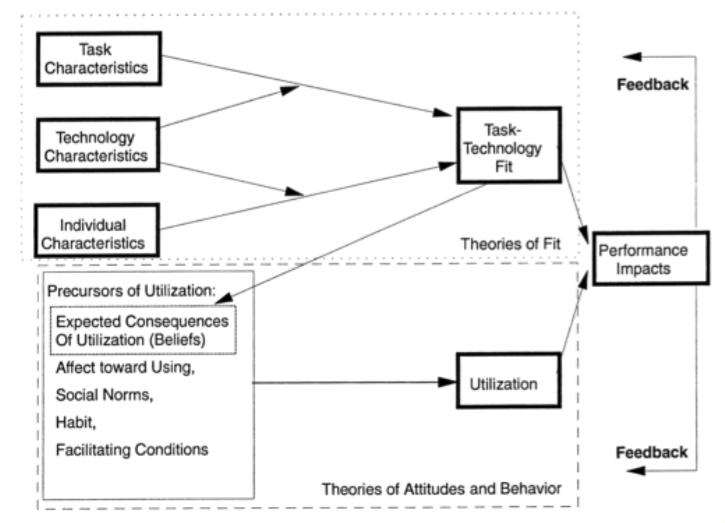
\includegraphics[width=\textwidth]{grafiken/ttf.png}
	\caption{Task-Technology Fit model\cite{MES10}}
\end{figure}

In case of the pilot stage of th Test Sheet in figo GmbH the properties of TTF model are following:
\paragraph{Task characteristics:}
\begin{itemize}
	\item Moving responsibility for test definition from developers to management staff
	\item Reduce the time for bugs allocation and fixation
\end{itemize}


\paragraph{Technology Characteristics:}
\begin{itemize}
	\item Asynchronous software
	\item Real-time software
\end{itemize}

\paragraph{Individual Characteristics:}
\begin{itemize}
	\item  No or little software development background
\end{itemize}


The initial assumption was that Test Sheets can be the most beneficial approach to define test steps for system behavior validation. This was done with following "first principles":
\paragraph{Task-Technology-Fit:}
\begin{itemize}
	\item Test Sheet is a representation for tests developed with the goal to combine the power and completeness of formal programming language with a representation that is easy to understand and work with even for people with little IT knowledge\cite{ts}.
	\item node.js is an asynchronous event-driven framework designed to build scalable network applications.
	\item Optimization for real-time execution is done by changing test steps execution order and position in the event loop with the respect to their reference structure
	\item Automatization of bug reporting process directly to the developer (not covered in paper probably should not be mentioned)
\end{itemize}

\paragraph{Utilization:}
\begin{itemize}
	\item User experience inherited from spread sheet editors;
	\item Simple conventions
\end{itemize}

\paragraph{Performance Impact:}
\begin{itemize}
	\item Better / automated quality assurance process
	\item Wider spread of tasks and responsibility distributions amongst developers and managers
	\item Increased awareness / technical understanding of product functionality for managers 
	\item Time for training and using the test sheet required from managers
	\item Change of job descriptions / new tasks and responsibilities for managers
\end{itemize}

\section{Benefits and affecting factors}
The factors influenced project's benefits were analyzed from the perspective of short term model (e. g. Functional fit, Overcoming organizational inertia).
\paragraph{Functional Fit} is the extent to which the functional capabilities are embedded and configured within an system package match the functionality that organization needs to operate effectively and efficiently.
\begin{itemize}
	\item reduced load of developers;
	\item reduced time to detect bug;
\end{itemize}

\paragraph{Overcoming Organizational Inertia} is the extent to which members of the organization have been motivated to learn, use, and accept new system. During initial implementation and subsequent upgrade projects, considerable change-management effort, training, and support are needed to overcome organizational inertia.
\begin{itemize}
	\item high attendance to the workshop and  results of user experience measurements showed wills of individuals for system's use within the everyday business process.
\end{itemize}

The benefits detected after the pilot stage of the Test Sheet project were classified  as \textit{operational}, \textit{managerial}, \textit{organizational} by their perspectives of the system's influence.

\paragraph{Operational Benefits:}
\begin{itemize}
	\item Feedback cycle time reduction;
	\item Productivity improvement - Developers can concentrate more on creating and fixing code instead of running manual tests
	\item Quality improvement - Errors are identified earlier due to automated monitoring, bugs are easier identified before deployments
	\item Customer Service improvement - Less complaints from customers (!not descriptive "LESS")
\end{itemize}

\paragraph{Managerial benefits:}
\begin{itemize}
	\item Resource management - No additional QA staff necessary
\end{itemize}


\paragraph{Organizational benefits} from the system use from the perspective of senior management, is an overall measure of senior managemt's perception of the benefits from the IT-based application. Such benefits usually revolve around the software enabling the faster and more accurate process of coordination and execution, resulting in more tightly controlled organizational processes improved asset utilization and decision making. \cite{MES11} 
Next organizational benefit were observed by chief technical and chief product managers during the use stage of the Test Sheet project:

\begin{itemize}
	\item Changing work patterns - Reduced workload on developers, increased product quality responsibility for managers
	\item Facilitating organizational learning - project mangers and customer support staff gain more technical understanding and feel empowered by owning the responsibility for the testing
\end{itemize}



\section{Misfits}
This section states the cases from the misfits' perspective of the software product implemented in scope of this research and the Test Sheet project. There are six perspectives where misfits can occur e. g. \textit{functionality, data, usability, role, control} and \textit{organizational culture} \cite{MES10}.

\paragraph{Functionality misfits:} occur, when the way processes are executed using the software leads to reduced efficiency and effectiveness compared to pre-ES outcomes. For this project no functionality misfits were detected.

\paragraph{Data misfits:}  occur, when data or its characteristics stored in or needed by the software leads to data quality issues such as inaccuracy, inconsistent representation, inaccessibility, lack of timeliness or inappropriateness for users' context. None of such cases was detected during system use.

\paragraph{Usability misfits:}  occur, when the interactions with the software required for task execution are cumbersome or confusing. During the system users' complains were generalized to the following statements: 
\begin{itemize}
	\item It is necessary to manually set define JSON object to be sent to API as well as object for an expected result;
	\item Test generated code must be copied to the same machine as working system (only for testing of scraping scripts)
	\item Code generation requires call execution of the command from the terminal.
\end{itemize}


\paragraph{Role misfits} occur, when the roles in the software are inconsistent with the skills available, create imbalances in the workload leading to bottlenecks and idle time, or generate mismatches between responsibility and authority. During the system's use none of such cases was detected.

\paragraph{Control misfits} occur, when the controls embedded in the software provide too much control, inhibiting productivity, or too little control, leading to the inability to assess or monitor performance appropriately. The only misfit detected from this perspective was identified on a project planning stage and was accepted as a necessary trade off by the technical management team:
\begin{itemize}
	\item Users need to have an access to the production version of the code base to define test cases;
\end{itemize}

\paragraph{Organizational culture misfits}  occur, when the software requires ways of operating that counterforce organizational norms. Within the system use period there was no users' or any other staff complains regrading any of this problems.


The most of misfits detected during the system use are related to the usability factor.
Input and output parameters JSON type required by the nature of system under test. This factor can by overcome by defining more convenient structure from the users' perspective and  adding internal translation from a new data type to JSON.
Generation of executable files as well as their deploying to the production environment planned to be done with background task which uses version control system's hooks.


Despite of the factors stated above the user experience is good. As well as TTF. This was achieved by Test Sheet approach itself. Event system of node.js. The approach taken for code generation which reduce idle time of the generated code and reporting mechanism (lays out of the scope of this paper). 
The benefits of the system use have showed themselves already during the pilot stage in all operational, managerial and organizational layers.
